\chapter{Traffic Science}

\section{Domain}

The road network can be represented with a \textbf{directed multi-graph} of intersections and roads. Each road has one or more lanes, a maximum speed and vehicles allowances dictating which kind of vehicles are allowed to flow through it. While more simplistic models use undirected graph with labelled edges to represent lanes and one/two-way traffic, it should be noted that a simple directed graph wouldn't be sufficient as in real-world road networks the may be more different links between an intersection. While some network slices could be represented with a single edge, there are more complex situations as in figure \ref{fig:multigraph-is-better-than-nothing} (a slice of Viale Zara, Milano, Italy) in which two big intersections are linked with two main one-way three-lane roads, two side one-way one-lane roads ("controviali") and two dedicated links for tramway vehicles. These roads are phisically separated with median strips and each link may allow for different turns within the intersections. Of course, the implementation model can be optimized for performance, but the logical model should remain a multi-graph because it represents better the features of the road network.

\textbf{Traffic} can be defined as a flow of vehicles on a network with peaks of density in some locations in which the average speed of those vehicles is significantly lower than the average of the entire network.
Each \textbf{vehicle} follows a path which can be influenced by its \textit{origin} and \textit{destination}, driving habits and knowledge, traffic conditions and usually also road regulations and transit/delivery plannings.
Mathematically speaking, \textbf{traffic} emerges when many vehicles need or want to transit through a shared path which hasn't enough capacity for handling this high number of users.
Urban planning authorities has since then taken this hint quite literally, incrementing the number of lanes year-by-year, but in the end the only result was an increase in road vehicles with unchanged transit density or, even worse, with higher travel times.
In this context, \textbf{traffic science} tries to analyze and model demand and road usage in order to identify the causes of traffic, optimize its regulation and eventually solving it.



\begin{figure}[t]
    \centering
    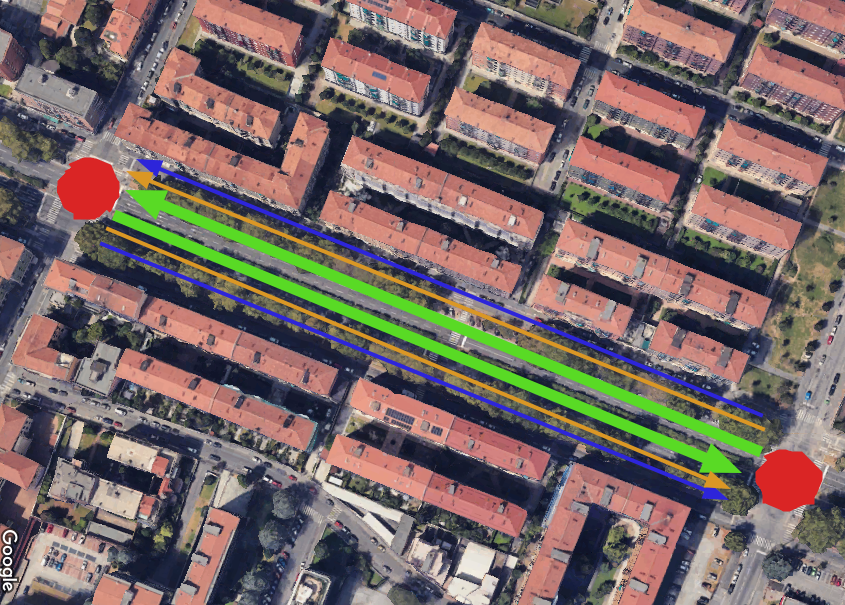
\includegraphics[width=0.75\linewidth]{figures/multigraph-is-better-than-nothing.png}
    \caption{A complex intersection pair which is connected with more different roads. Viale Zara. Milano. Italy}
    \label{fig:multigraph-is-better-than-nothing}
\end{figure}

\section{Demand models}

\section{Assumptions}

\section{Scenarios}
